\subsection{System Architecture}
To help D-FLAT profit from machine learning techniques an architecture based on the architecture proposed in ~\cite{DBLP:conf/lpnmr/GebserKKSSZ11} was used. The architecture is shown in Figure~\ref{impl:sysarch}. First instance features are extracted, then a prediction which solver configuration will be the best is made using machine learning algorithms and finally D-FLAT is launched with the predicted configuration.
\begin{figure}[h]
	\center
	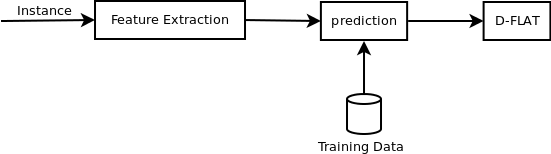
\includegraphics[scale=0.6]{figures/sysarch.png}
	\caption{System Architecture of D-FLAT with Learning\label{impl:sysarch}}
\end{figure}
A python script was implemented to handle the control flow such that the user only has to supply the instance and learning database. Furthermore some modifications to D-FLAT were made to allow the configuration of the solver.

\subsection{Modifications to D-FLAT}
To the default configuration four different clasp configurations were added using \lstinline$clasp_fascade$ of its library. The three configurations \emph{jumpy},\emph{frumpy},\emph{crafty} aim to rebuild the portfolios provided by clasp, while \emph{nopre} instructs clasp to skip any preprocessing and start solving directly. These configurations where added to the \lstinline$Asp$ class in D-FLAT. Users can set the desired portfolio by using the \lstinline$--portfolio$ flag followed by the name of the portfolio in the command line arguments.

Another new flag \lstinline$--ext-feat$ instructs D-FLAT to stop processing after decomposing the instance and print out its decomposition width in machine readable format. This flag is used for feature extraction. Additional feature extractors can be implemented by writing subclasses of \lstinline$FeatureExtractor$ and adding corresponding instances to the list \lstinline$felist$ in the $Algorithm$ class.

\subsection{Learner}
Learner is a python script capable of building a learning base for the machine learning as well as performing machine learning algorithms itself. It is configured by command line arguments as well as an xml configuration file. If it is used without any command line arguments it attempts to build a learning base made of instances read from \lstinline$config.xml$. More details will be given in benchmarks~\ref{sec:benchmarks}.

Usage of the command line flag \lstinline$-p$ or \lstinline$--predict$ together with an instance as well as problem encoding and a learning base will launch in Learner in prediction mode. It will try to predict the best solver configuration based on the supplied learning base and launch D-FLAT with the predicted config. Using $--help$ gives the full list of commands, which can also be seen in Listing~\ref{lst:learnercmd}.
\begin{lstlisting}[label=lst:learnercmd]
TODO
\end{lstlisting}

